\section{Перенос в постоянном равномерном поле скоростей}

Скорость принимается постоянной на всем пространстве с течением времени. Источник нулевой, начальной распределение --- функция-шапочка:

\begin{equation}
	v = const
\end{equation}


\begin{equation}
	f(x,t) \equiv 0
\end{equation}

\begin{equation}
	\phi(x) = \exp\left(-\frac{a^2}{a^2 - \left(x-b\right)^2} + 1\right)
\end{equation}

При $\alpha = 1$ получаем обычное уравнение переноса. Численное решение принимает вид:

\begin{figure}[h]
	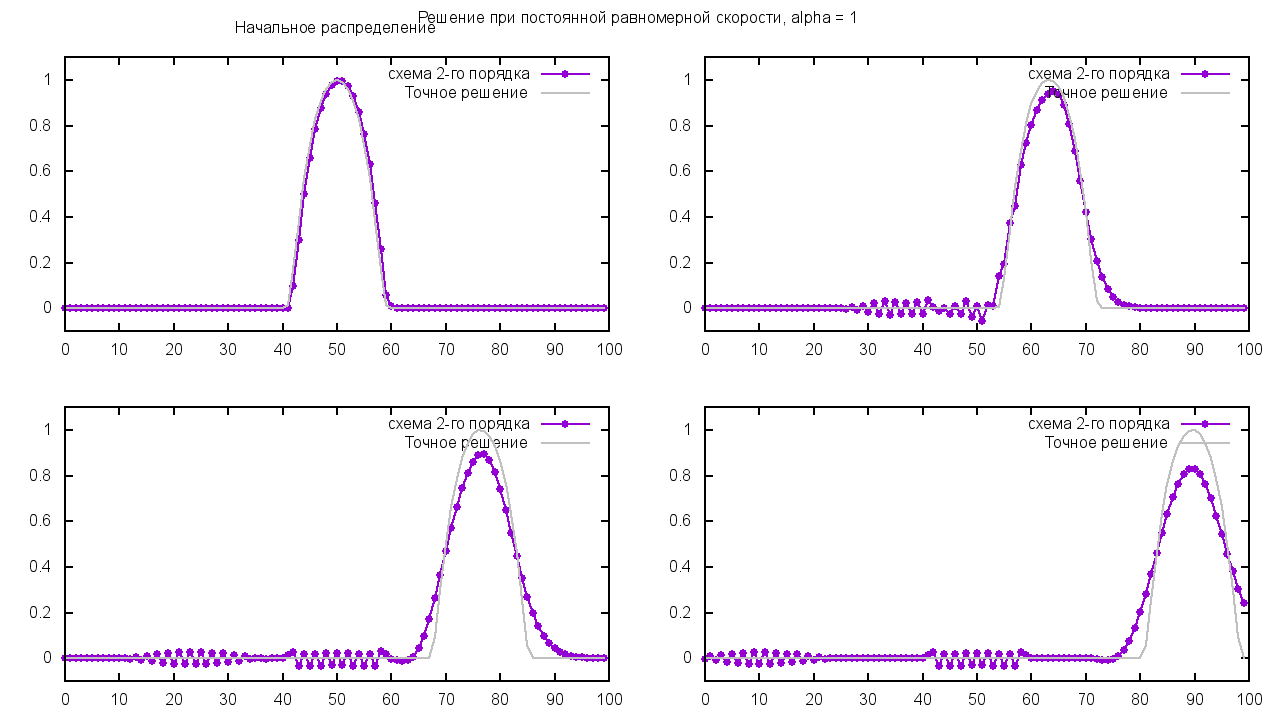
\includegraphics[width=1.2\linewidth]{pics/alpha1_notvd}
	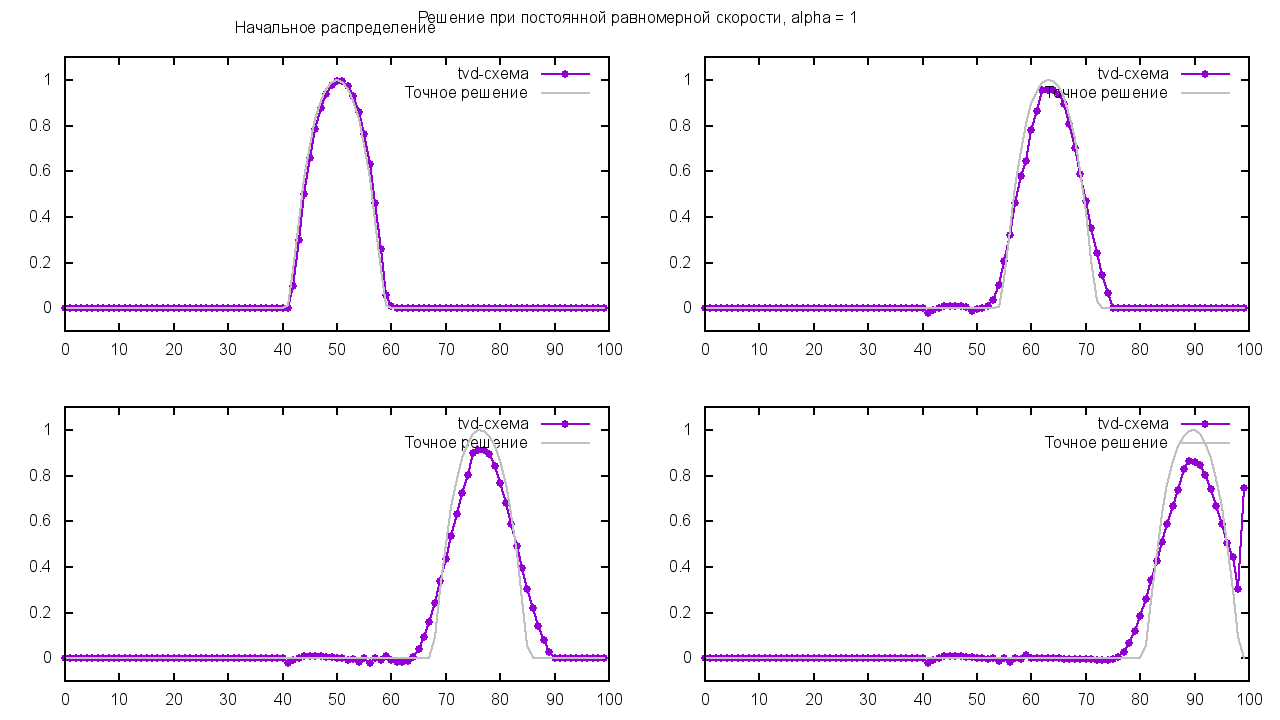
\includegraphics[width=1.2\linewidth]{pics/alpha1_tvd}
\end{figure}

Для дробного $\alpha = 0.9$ была применена та же TVD-схема, получены решения

\begin{figure}
	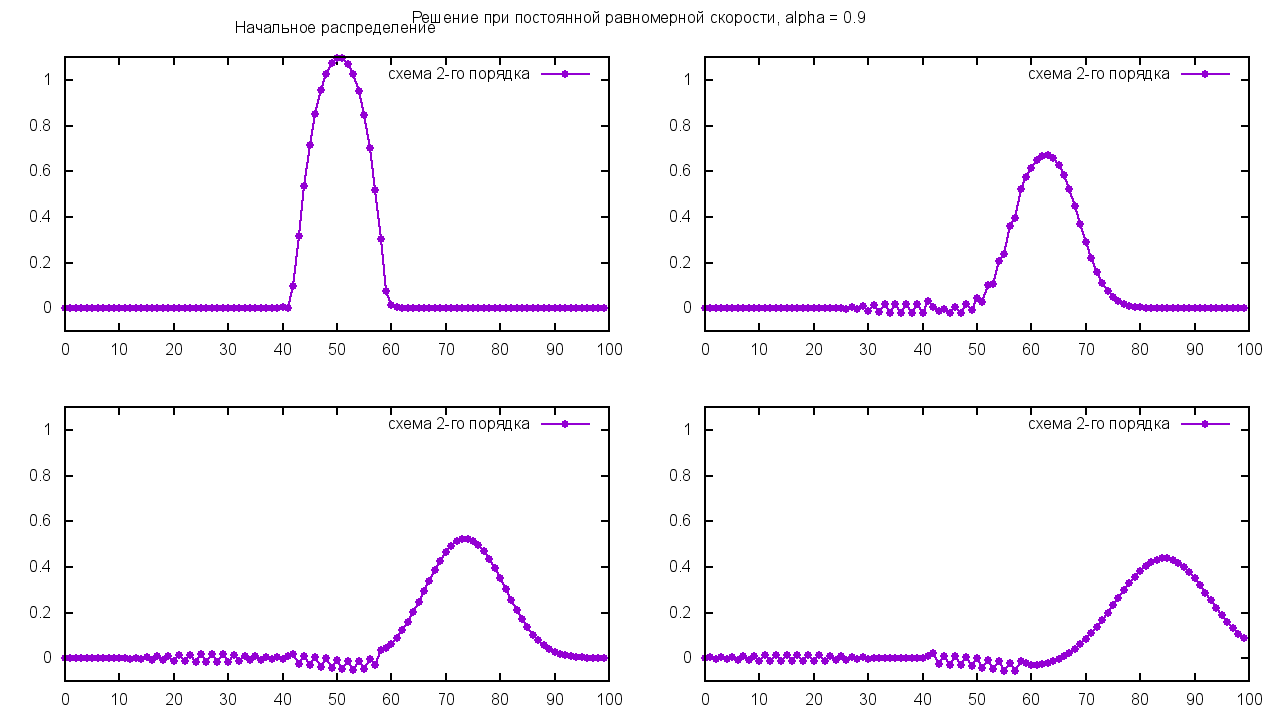
\includegraphics[width=1.2\linewidth]{pics/alpha09_notvd}
	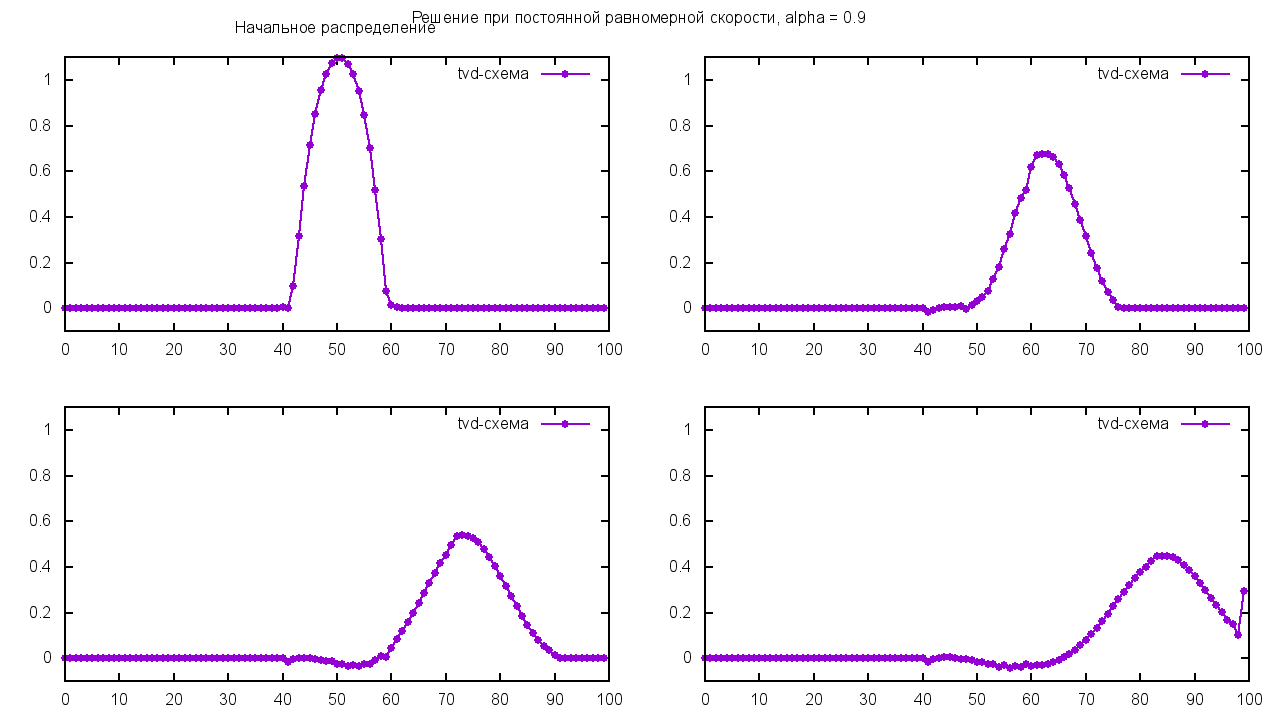
\includegraphics[width=1.2\linewidth]{pics/alpha09_tvd}
\end{figure}

Также получены решения для $\alpha = 0.7$:

\begin{figure}
	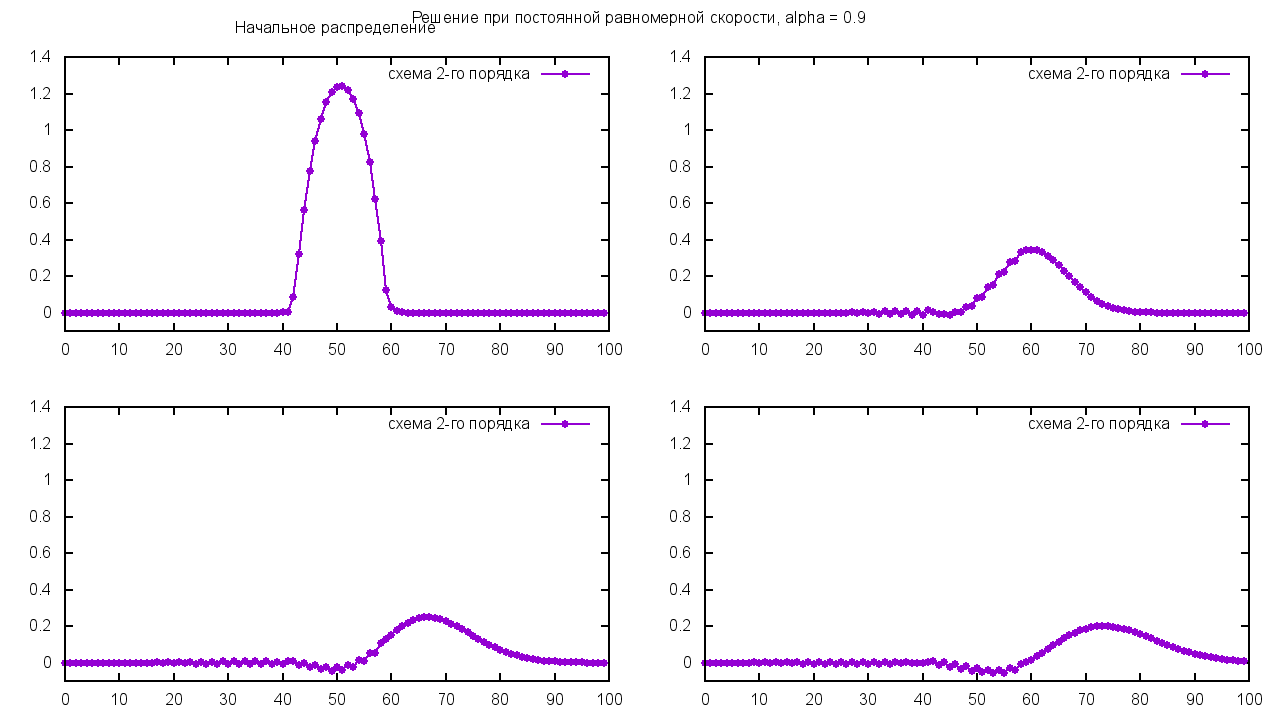
\includegraphics[width=1.2\linewidth]{pics/alpha07_notvd}
	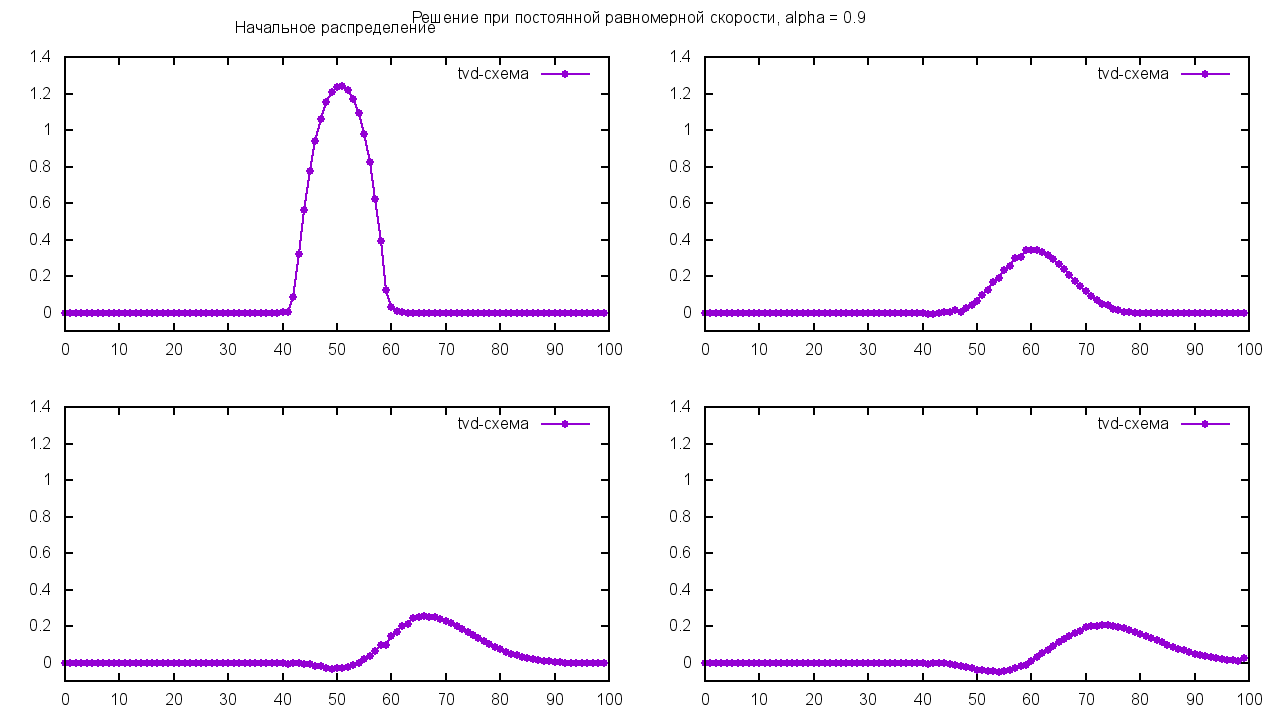
\includegraphics[width=1.2\linewidth]{pics/alpha07_tvd}
\end{figure}

Также получены решения для $\alpha = 0.5$:

\begin{figure}
	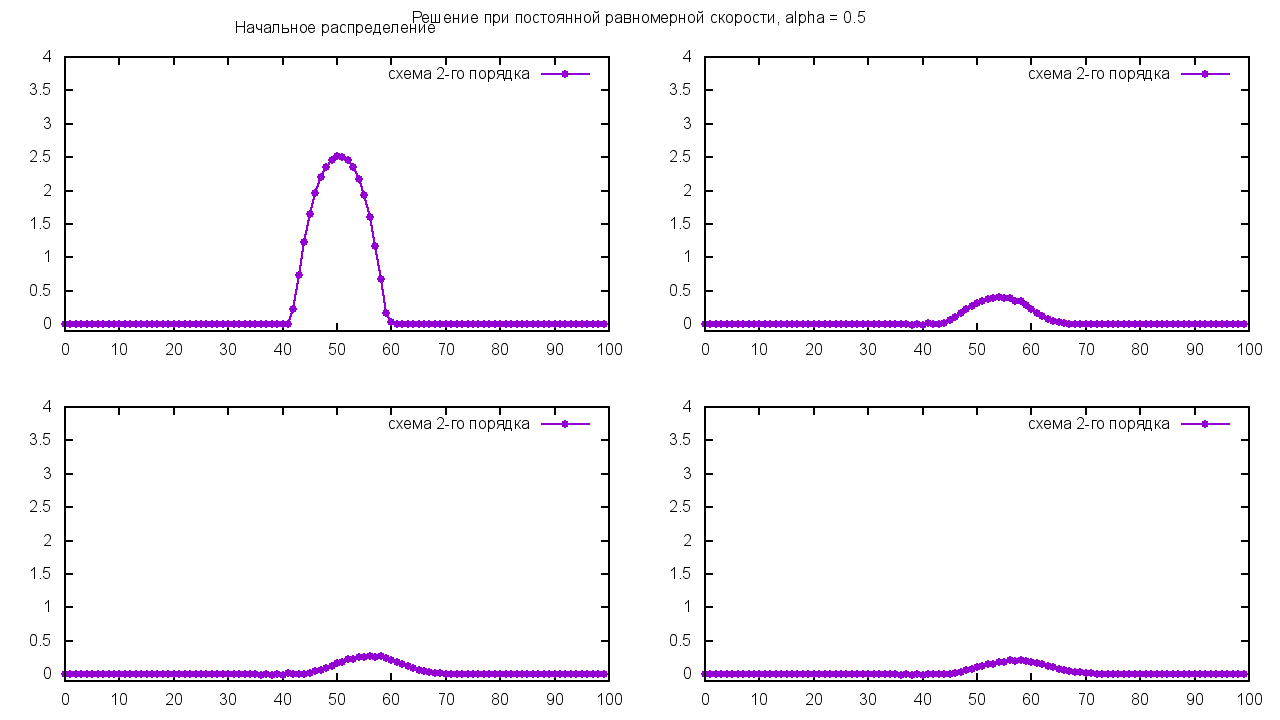
\includegraphics[width=1.2\linewidth]{pics/alpha05_notvd}
	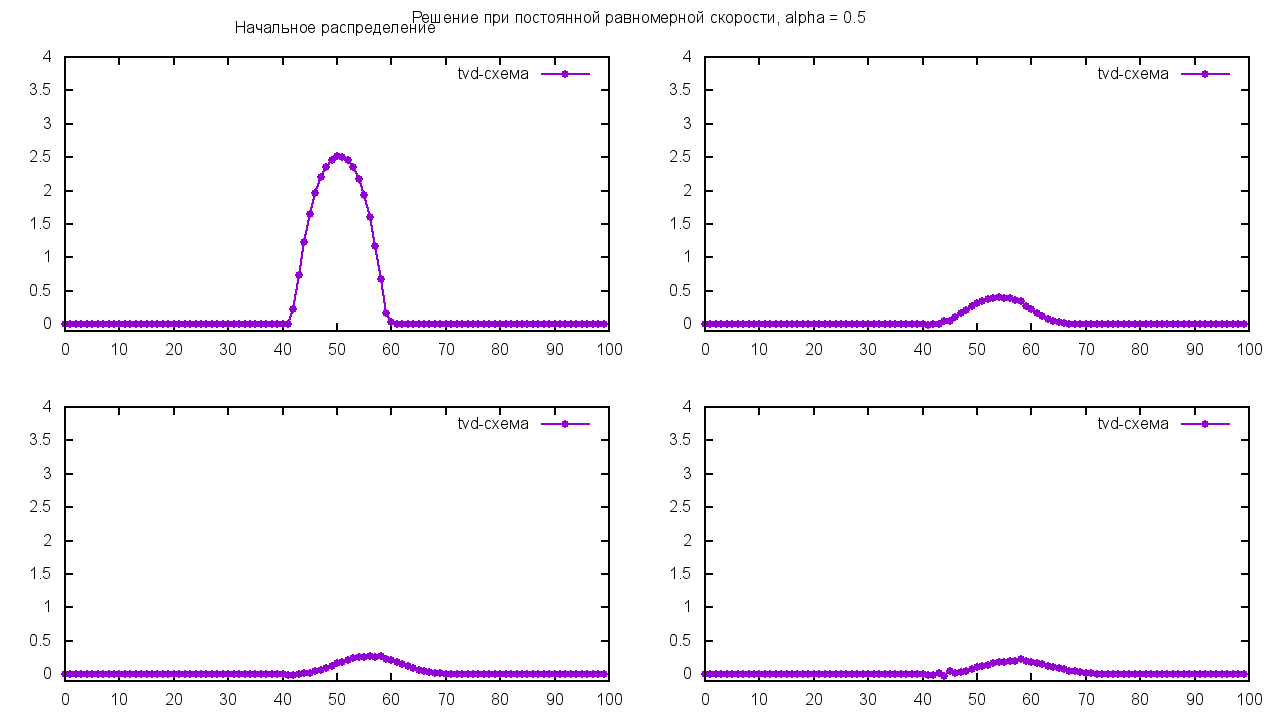
\includegraphics[width=1.2\linewidth]{pics/alpha05_tvd}
\end{figure}
